\section{Технологический раздел}

\subsection{Выбор средств программной реализации}

В качестве языка программирования был выбран Python, так как:

\begin{itemize}
	\item[---] имеется достаточный опыт программирования на этом языке, что сократит время написания программы;
	\item[---] для данного языка программирования имеются все необходимые библиотеки для работы с байесовскими моделями и аудиофайлами, что также ускорит процесс разработки.
\end{itemize}

В качестве среды разработки был выбран PyCharm по следующим причинам:

\begin{itemize}
	\item[---] он бесплатен для использования студентами;
	\item[---] он имеет множество встроенных интсрументов, которые облегчают процесс написания и отладки кода;
	\item[---] имеется достаточный опыт программирования с использованием данной среды разработки, что сократит время изучения возможностей.
\end{itemize}

Для работы с аудиофайлами использовалась библиотека librosa~\cite{librosa}, а для реализации байесовских моделей -- библиотека PyMC3~\cite{pymc3_docs}. Кроме того в программе вместо обычных списков часто для удобства использовались numpy массивы~\cite{numpy}.

\subsection{Детали реализации}

\subsubsection{Байесовские модели}

В листингах \ref{lst:bpmmodel}, \ref{lst:measuremodel} представлена реализация байесовских иерархических моделей для оценки темпа и тактового размера соответственно.

\newpage

\begin{lstlisting}[label={lst:bpmmodel}, caption={реализация байесовской модели для определения темпа}]
	def bpm_model(min_bpm: int, max_bpm: int, bpm_dataset, genre_dataset, genres_ints, progress):
		with pm.Model() as model:
			# hyperpriors (lvl 1)
			tempo = pm.Uniform('tempo', lower=min_bpm, upper=max_bpm)
			progress.setValue(20)
			mu = (min_bpm + max_bpm) / 2.0
			sigma = (max_bpm - min_bpm) / 12.0
			genre_coef = pm.Normal('genre_coef', mu=0, sd=1, shape=len(genre_dataset.unique()))
			progress.setValue(40)
	
			# prior (lvl 2)
			bpm_est = mu + genre_coef[genres_ints] * sigma
			progress.setValue(60)
	
			# likelihood (lvl 3)
			bpm_obs = pm.Normal('bpm_obs', mu=bpm_est, sd=sigma, observed=bpm_dataset)
			progress.setValue(80)
	
			# get the samples
			trace = pm.sample(1000, tune=500, chains=2, cores=1)
			progress.setValue(100)
	
		return trace
\end{lstlisting}

\begin{lstlisting}[label={lst:measuremodel}, caption={реализация байесовской модели для определения ритма}]
	def rhythm_model(measure_min, measure_max, rhythm_dataset, progress):
		with pm.Model() as model:
			# prior
			measure = pm.Uniform('measure', lower=measure_min, upper=measure_max)
			progress.setValue(20)
			mu = (measure_min + measure_max) / 2.0
			progress.setValue(40)
			sigma = (measure_max - measure_min) / 12.0
			progress.setValue(60)
			# likelihood
\end{lstlisting}

\begin{lstlisting}
			measure_obs = pm.Normal('measure_obs', mu=mu, sd=sigma, observed=rhythm_dataset)
			progress.setValue(80)

			trace = pm.sample(1000, tune=1000, chains=2)
			progress.setValue(100)
	
		return trace
\end{lstlisting}

На вход моделей поступают границы темпа или размера, массив значений из датасета (для оценки темпа -- это темпы и жанры, для ритма -- размеры), список жанров, закодированных числами (для темпа) (для размещения коэффициентов по индексам жанров) и линия прогресса из интерфейса для ее обновления.

Выходными данными указанных функций являются распределения соответствующих параметров (в первом случае -- это темп и коэффициенты для всех жанров, а во втором -- тактовый размер).

Метод sample отвечает за сам процесс моделирования (получения апостериорных распределений).

Расчет диапазона возможных темпов был реализован с помощью метода beat\_track() из библиотеки librosa, в качестве дельты взято 40 bpm.

\subsubsection{Разделение аудиофайла}

В листинге \ref{lst:splitaudio} представлена реализация функции разделения аудиофайла на фрагменты.

\begin{lstlisting}[label={lst:splitaudio}, caption={разделение аудиофайла на фрагменты}]
	def split_mp3(audio_path: str, step: int):
		if not os.path.isdir("tmp"):
			os.mkdir("tmp")
		# load audio
		audio_file = AudioSegment.from_file(audio_path, format="mp3")
		# fragments length in milliseconds
		part_length = step
\end{lstlisting}

\begin{lstlisting}
		# split audio
		parts = [audio_file[i:i + part_length] for i in range(0, len(audio_file), part_length)]
		# save fragments
		for i, part in enumerate(parts):
			part.export(f"tmp/part_{i}.mp3", format="mp3")
\end{lstlisting}

Функция создает временную директорию <<tmp/>>, в которую впоследствии сохраняет фрагменты указанного аудиофайла в формате mp3. После расчета темпов или размеров для всех фрагментов созданная директория очищается и удаляется.

\subsubsection{Определение диапазона размеров}

В листинге~\ref{lst:measurerange} представлена реализация функций для расчета диапазона размеров.

\begin{lstlisting}[label={lst:measurerange}, caption={определение диапазона размеров}]
	def calc_measure(downbeats: list) -> int:
		downbeat_inds = [i for i, beat in enumerate(downbeats) if beat == 1]
		if len(downbeat_inds) <= 1:
			return 0
		difs_sum = 0
		for i in range(1, len(downbeat_inds)):
			difs_sum += (downbeat_inds[i] - downbeat_inds[i - 1])
		avg_measure = difs_sum / (len(downbeat_inds) - 1)
		return round(avg_measure)
	
	def get_measure_range(audio_path: str, tail: list):
		y, sr = librosa.load(audio_path)
		onset_env = librosa.onset.onset_strength(y=y, sr=sr)
		# amplitude peaks
		peaks = librosa.util.peak_pick(onset_env, pre_max=3, post_max=3, pre_avg=3,
		post_avg=5, delta=0.5, wait=10)
		peaks_time = librosa.frames_to_time(peaks, sr=sr)
		_, beats = librosa.beat.beat_track(onset_envelope=onset_env, sr=sr)
		beats_time = librosa.frames_to_time(beats, sr=sr)
\end{lstlisting}

\begin{lstlisting}
		# beginnings of bars
		downbeat_times = {}
		for i, beat in enumerate(beats_time):
		if beat in peaks_time:
		downbeat_times[i] = beat
		downbeats = [0 for i in range(len(beats))]
		for beat in downbeat_times.keys():
		downbeats[beat] = 1
		downbeats = tail + downbeats
		prior_measure = calc_measure(downbeats)
		if prior_measure == 0:
			return -1, downbeats
		if prior_measure > 2:
			return 0, np.arange(prior_measure - 2, prior_measure + 3, 1)
		elif prior_measure == 2:
			return 0, np.arange(prior_measure - 1, prior_measure + 3, 1)
		else:
			return 0, np.arange(prior_measure, prior_measure + 3, 1)
\end{lstlisting}

Функция calc\_measure отвечает за расчет тактового размера на основе списка из чередующихся сильных и слабых долей, где сильные доли обозначаются 1, а слабые -- 0.

Если в указанном отрывке найдена только одна сильная доля, то этот фрагмент объединяется со следующим. Для этого среди входных данных функции get\_measure\_range есть параметр tail, который представляет собой список сильных и слабых долей предыдущего фрагмента аудио.

Набор сильных долей формируется на основе совпадений времени в двух списках: пиков амплитуды (peaks\_time) и <<ударов>> (beats\_time).

\subsection{Пользовательский интерфейс}

На рисунке~\ref{img:gui} представлен интерфейс разработанного приложения.

Приложение поддерживает загрузку только mp3 файлов. Список возможных жанров загружаемой музыки был создан на основе датасета. Темпы и размеры можно определять отдельно, независимо друг от друга.

\begin{figure}[h]
	\centering
	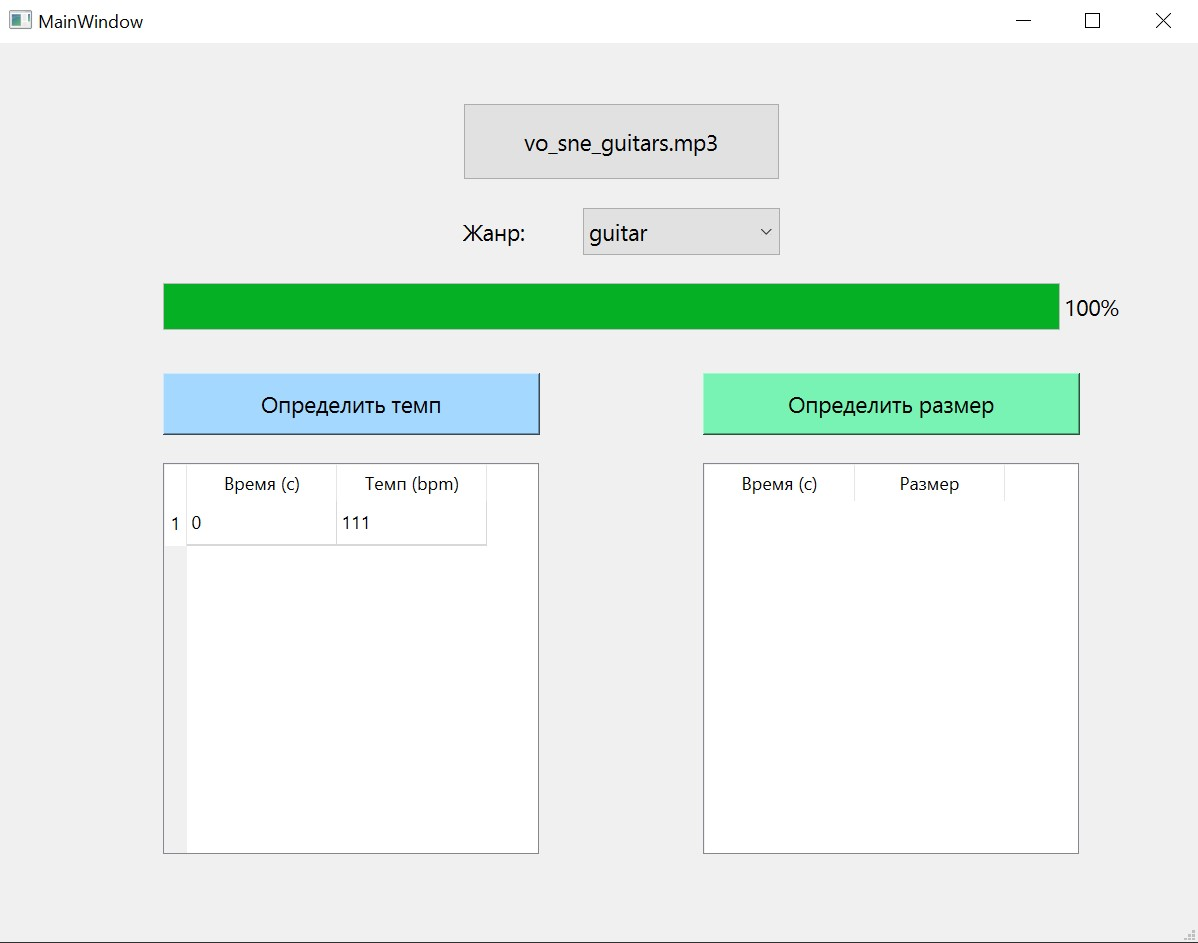
\includegraphics[scale=0.7]{inc/img/gui.jpg}
	\caption{Интерфейс приложения}
	\label{img:gui}
\end{figure}

Для того, чтобы определить темп аудиофайла, необходимо:

\begin{enumerate}
	\item Загрузить аудиофайл, нажав на верхнюю кнопку.
	\item Выбрать жанр загруженной музыки из выпадающего списка ниже.
	\item Нажать на кнопку <<Определить темп>>.
	\item Результаты появятся в левой таблице через 1,5-2 минуты.
\end{enumerate}

Для определения ритма:

\begin{enumerate}
	\item Загрузить аудиофайл, нажав на верхнюю кнопку.
	\item Нажать на кнопку <<Определить размер>>.
	\item Результаты появятся в правой таблице в течение минуты.
\end{enumerate}

Жанр в этом случае указывать необязательно.

\newpage

\subsection{Тестирование приложения}

В процессе разработки приложения проводились модульные тесты (листинг~\ref{lst:units}). Тестировались такие функции, как: разделение аудиофайла на фрагменты, очистка директории, удаление директории и расчет тактового размера на основе списка сильных и слабых долей.

\begin{lstlisting}[label={lst:units}, caption={модульные тесты}]
	class SplitAudio(unittest.TestCase):
		def test_splitting(self):
			audio = "test_audio/vo_sne.mp3"
			step = 5000
			split_mp3(audio, step)
			self.assertEqual(os.path.exists("tmp/"), True)
			self.assertGreater(len(os.listdir("tmp/")), 0)
	
	class CleanDirs(unittest.TestCase):
		def test_cleaning(self):
			os.mkdir("temp/")
			fp = open('temp/file.txt', 'x')
			fp.close()
			dir = "temp/"
			clean_dir(dir)
			self.assertEqual(len(os.listdir(dir)), 0)
			os.rmdir(dir)
		def test_removing(self):
			os.mkdir("temp/")
			dir = "temp/"
			remove_dir(dir)
			self.assertEqual(os.path.exists("temp/"), False)
	
	class CalcMeasure(unittest.TestCase):
		def test_calculating(self):
			downbeats = [1, 0, 0, 0, 1, 0, 0, 0, 1]
			measure = calc_measure(downbeats)
			self.assertEqual(measure, 4)
\end{lstlisting}

Как видно из рисунка~\ref{img:units}, все модульные тесты были успешно пройдены.

\begin{figure}[h]
	\centering
	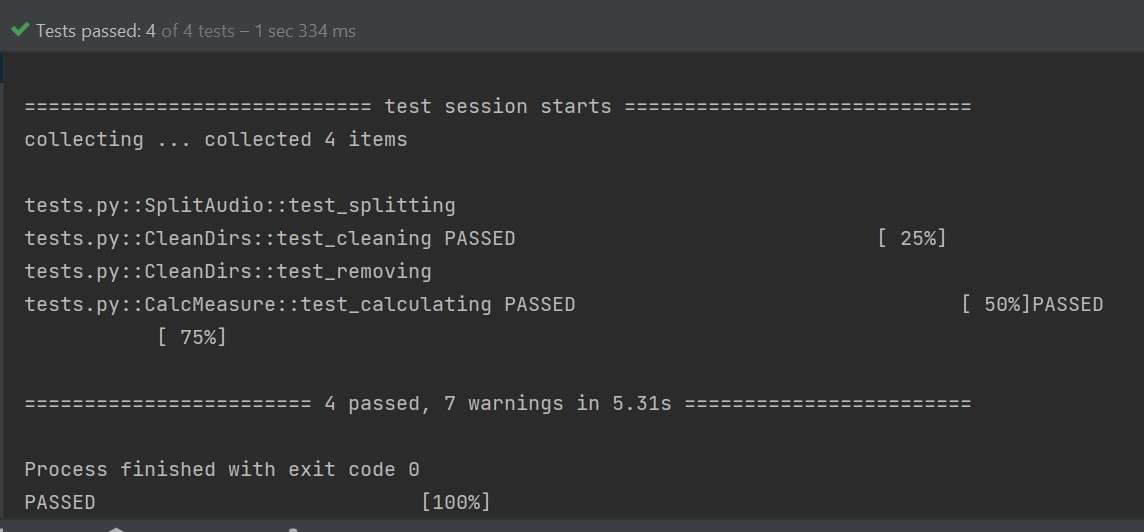
\includegraphics[scale=0.8]{inc/img/units.jpg}
	\caption{Результаты модульного тестирования}
	\label{img:units}
\end{figure}

\newpage

Работоспособность программы в целом проверялась вручную. На рисунке~\ref{img:test_const} представлены результаты работы программы на одном из аудиофайлов.

\begin{figure}[h]
	\centering
	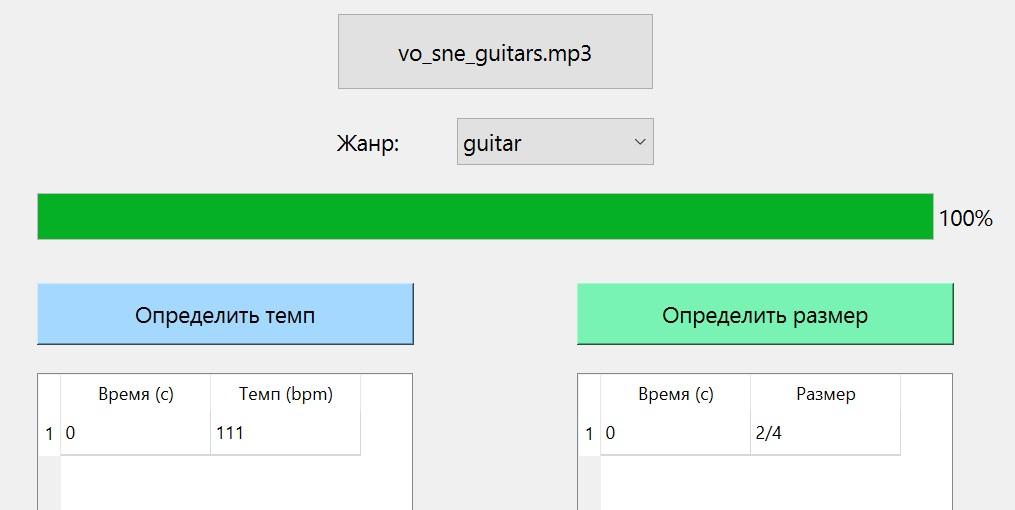
\includegraphics[scale=0.9]{inc/img/test_constant.jpg}
	\caption{Результаты для постоянного темпа и ритма}
	\label{img:test_const}
\end{figure}

\newpage

При этом заранее известно, что темп данной аудиозаписи 125 bpm, а тактовый размер -- 4/4 (рис.~\ref{img:vosne_ref}, самое левое число -- темп в bpm, правее -- размер).

\begin{figure}[h]
	\centering
	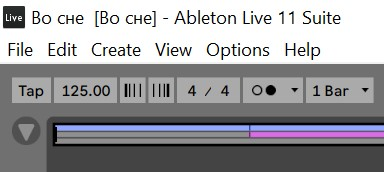
\includegraphics[scale=1.4]{inc/img/vosne_ref.jpg}
	\caption{Эталонные значения темпа и размера}
	\label{img:vosne_ref}
\end{figure}

Таким образом, отклонение полученного темпа от идеального составляет примерно 11\%, что является приемлемым результатом, поскольку согласно исследованиям~\cite{bayesian} ошибки байесовского метода могут составлять до 18\%.

Размер 2/4 также является допустимым результатом в данном случае. Это означает, что сильных долей в аудиозаписи было выявлено в два раза больше, но при этом основной ритм остается тем же, что и при 4/4 (т.~к. два такта по 2/4 дают в сумме один такт с размером 4/4).

Для тестирования определения переменного темпа использовался аудиофайл с темпом 115 bpm в первые 25 секунд и 120 bpm в оставшееся время (размер этого музыкального фрагмента постоянен и равен 6/8, что в данном случае может быть приравнено к 3/4).

Результаты работы метода представлены на рисунке~\ref{img:test_tempo}.

Ошибка определения темпа в данном случае составляет примерно 7\%, что также укладывается в допустимые пределы.

Для тестирования определения переменного ритма использовался аудиофайл с размером 3/4 в первые 15 секунд и 4/4 bpm в оставшееся время (темп этого музыкального фрагмента постоянен и равен 100 bpm).

Результаты работы метода представлены на рисунке~\ref{img:test_rhythm}.

Ошибка определения размера в таком случае составляет примерно 8\%.

\begin{figure}[h]
	\centering
	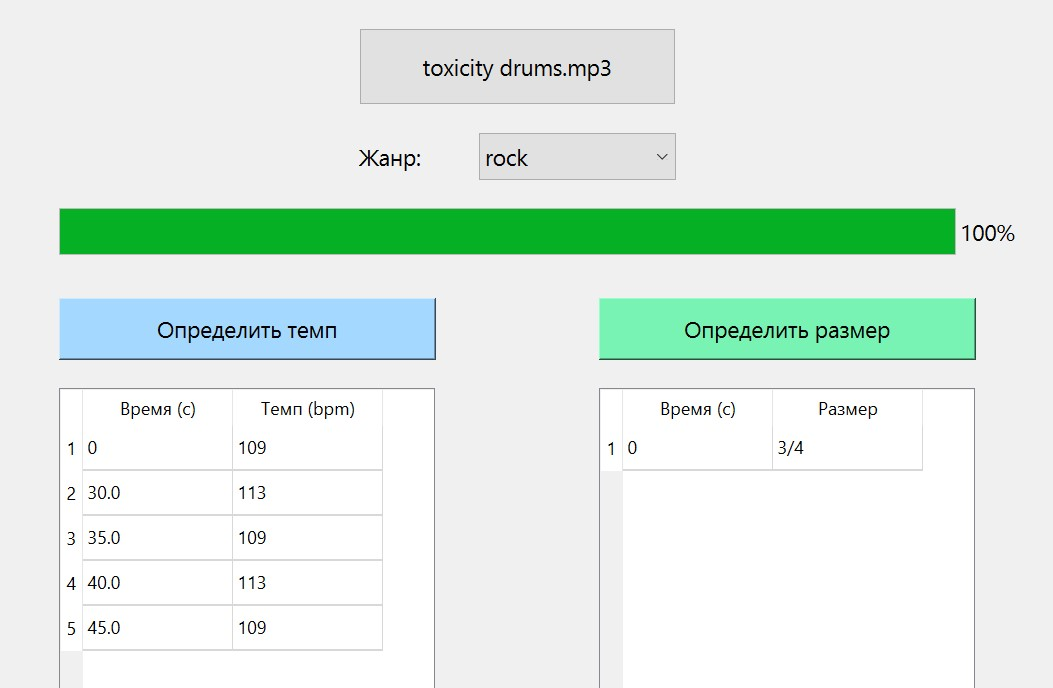
\includegraphics[scale=0.85]{inc/img/test_tempo.jpg}
	\caption{Результаты для переменного темпа}
	\label{img:test_tempo}
\end{figure}

\begin{figure}[h]
	\centering
	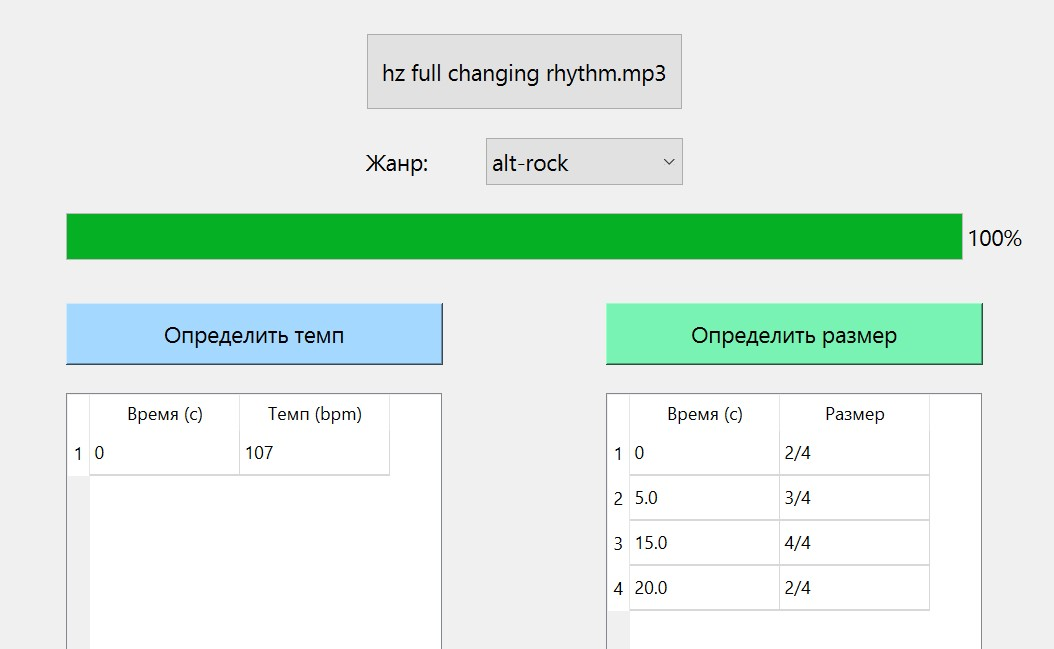
\includegraphics[scale=0.85]{inc/img/test_rhythm.jpg}
	\caption{Результаты для переменного размера}
	\label{img:test_rhythm}
\end{figure}

\clearpage

\subsection*{Выводы}

В данном разделе были выбраны язык программирования и среда разработки, а также приведены детали реализации, пользовательский интерфейс и результаты тестирования разработанной программы.

В качестве языка программирования был выбран Python, а в качестве среды разработки -- PyCharm.

Была описана реализация байесовских моделей для определения ритма и темпа, разделения аудиофайла на фрагменты и определения диапазона размеров.

Все модульные тесты были успешно пройдены. Результаты функциональных тестов также оказались в пределах допустимости.
